\documentclass[pdflatex,compress]{beamer}

%\usetheme[dark,framenumber,totalframenumber]{ElektroITK}
\usetheme[darktitle,framenumber,totalframenumber]{ElektroITK}
\usepackage{graphicx}
\usepackage{multicol}

\title{Data Communications}
\subtitle{Chapter 7 - Flow and Error Control}

\author{Mifta Nur Farid}

\begin{document}

\maketitle

\begin{frame}
	\frametitle{Data Link Control Protocols}
	\begin{itemize}
		\item Requirements and objectives for effective data communication between two directly connected transmitting-receiving stations:
		\begin{enumerate}
			\item Frame synchronization
			\item Flow control
			\item Error control
			\item Addressing
			\item Control and data
			\item Link management
		\end{enumerate}
	\end{itemize}
\end{frame}

\begin{frame}
	\frametitle{Flow Control}
	\begin{itemize}
		\item Technique for assuring that a transmitting entity does not over-whelm a receiving entity with data
		\item In the absence of flow control, the receiver’s buffer may fill up and overflow while it is processing old data
	\end{itemize}
\end{frame}

\begin{frame}
	\frametitle{Model of Frame Transmission}
	\begin{center}
		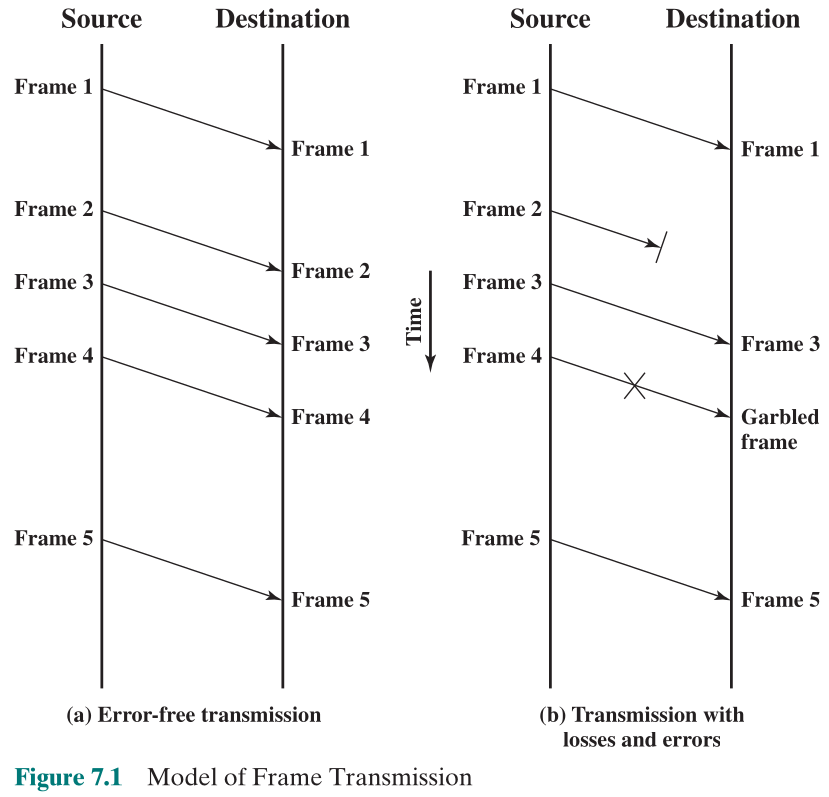
\includegraphics[width=0.6\linewidth]{img/img01}
	\end{center}
\end{frame}

\begin{frame}
	\frametitle{Stop-and-Wait Flow Control}
	\begin{itemize}
		\item Simplest form of flow control
		\begin{enumerate}
			\item Source transmits frame
			\item Destination receives frame and replies with acknowledgement (ACK)
			\item Source waits for ACK before sending next frame
			\item Destination can stop flow by not send ACK
		\end{enumerate}
	\end{itemize}
\end{frame}

\begin{frame}{Stop-and-Wait Flow Control}
	\begin{itemize}
		\item It is often the case that a source will break up a large block of data into smaller blocks and transmit the data in many frames
		\begin{itemize}
			\item The buffer size of the receiver may be limited
			\item The longer the transmission, the more likely that there will be an error, necessitating retransmission of the entire frame
			\item On a shared medium it is usually desirable not to permit one station to use the medium for an extended period, thus causing long delays at the other sending station
		\end{itemize}
	\end{itemize}
\end{frame}

\begin{frame}{Stop-and-Wait Link Utilization}
	\begin{center}
		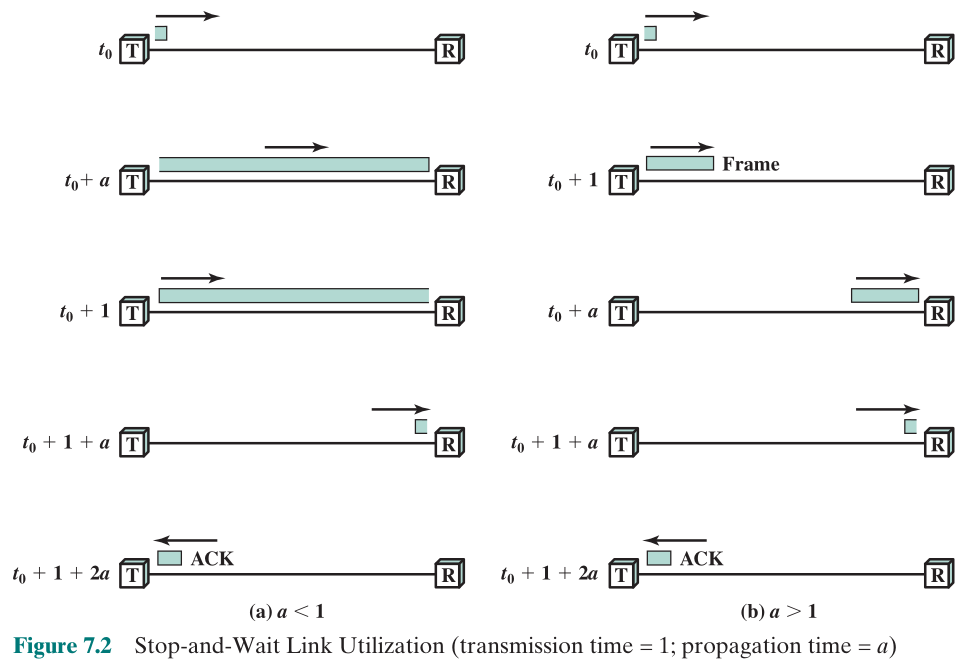
\includegraphics[width=0.9\linewidth]{img/img02}
	\end{center}
\end{frame}

\begin{frame}
	\frametitle{Sliding Windows Flow Control}
	\begin{itemize}
		\item Allows multiple numbered frames to be in transit
		\begin{itemize}
			\item Receiver has \textbf{buffer W} long
			\item Transmitter sends up to W frames without ACK
			\item \textbf{ACK includes number} of next frame expected
			\item \textbf{Sequence number} is bounded by \textbf{size of field (k)}
			\begin{itemize}
				\item Frames are numbered modulo $ 2^k $
				\item \textbf{Giving max window size of up to $ 2^k - 1 $}
			\end{itemize}
			\item Receiver can ACK frames without permitting further transmission (Receive Not Ready)
			\item Must send a normal acknowledge to resume
		\end{itemize}
		\item If have full-duplex link, can piggyback ACKs
	\end{itemize}
\end{frame}

\begin{frame}
	\frametitle{Sliding Window Diagram}
	\begin{flushright}
		3-bit seq, W = 7 frames
	\end{flushright}
	\begin{center}
		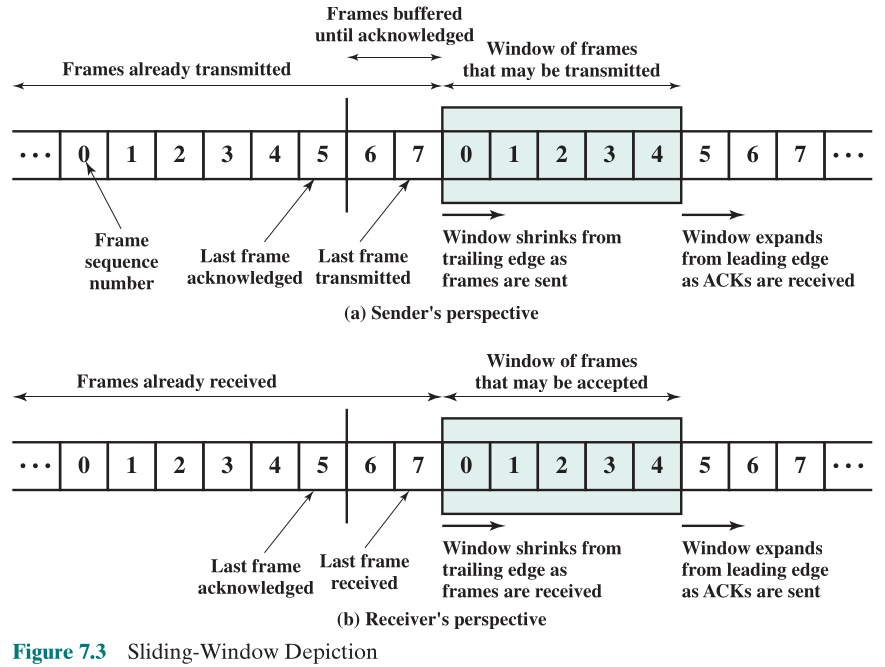
\includegraphics[width=0.8\linewidth]{img/img03}
	\end{center}
\end{frame}

\begin{frame}
	\frametitle{Sliding Window Example}
	\begin{center}
		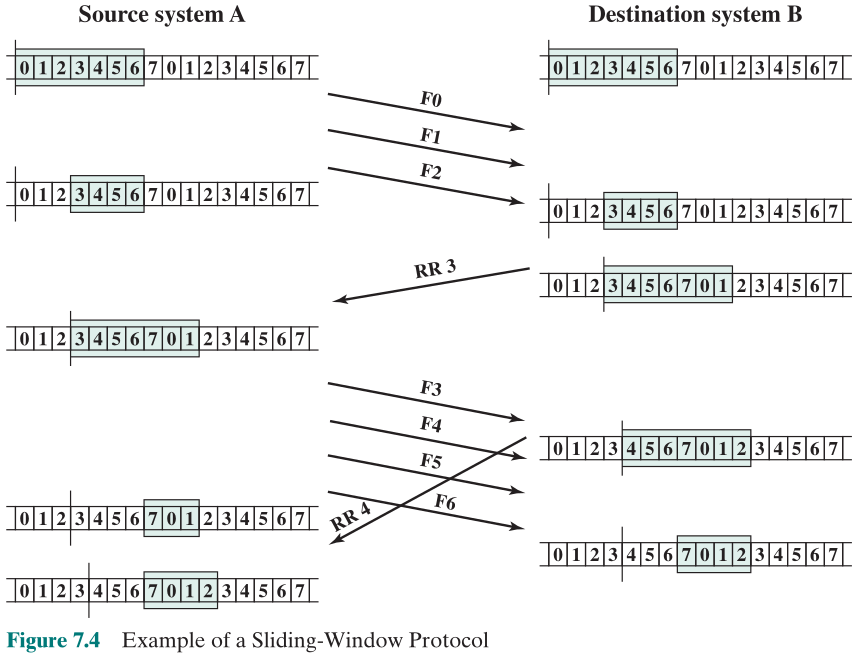
\includegraphics[width=0.8\linewidth]{img/img04}
	\end{center}
\end{frame}

\begin{frame}
	\frametitle{Sliding Window Utilization}
	\begin{itemize}
		\item Window size $ W $, transmission time = 1, propagation time = $ a $
		\item Case 1: $ W >= 2a + 1 $
		\begin{itemize}
			\item Sender A can transmit continuously with no pause and normalized throughput is 1.0
		\end{itemize}
		\item Case 2: $ W < 2a + 1 $
		\begin{itemize}
			\item Sender A exhausts its window at $ t = W $ and cannot send additional frames until $ t = 2a + 1 $.
			\item Normalized throughput is $ W/(2a+1) $
		\end{itemize}
	\end{itemize}
\end{frame}

\begin{frame}
	\frametitle{Error Control Techniques}
	\begin{itemize}
		\item Detection and correction of errors such as:
		\begin{itemize}
			\item Lost frames: a frame fails to arrive at the other side
			\item Damaged frames: frame arrives but some of the bits are in error
		\end{itemize}
		\item Common techniques use:
		\begin{itemize}
			\item Error detection
			\item Positive acknowledgment
			\item Retransmission after timeout
			\item Negative acknowledgement \& retransmission
		\end{itemize}
	\end{itemize}	
\end{frame}

\begin{frame}
	\frametitle{Automatic Repeat Request (ARQ)}
	\begin{itemize}
		\item Collective name for error control mechanisms, including:
		\begin{itemize}
			\item stop and wait
			\item go back N
			\item selective reject (selective retransmission)
		\end{itemize}
		\item Effect of ARQ is to turn an unreliable data link into a reliable one
	\end{itemize}
\end{frame}

\begin{frame}
	\frametitle{Stop and Wait ARQ}
	\begin{itemize}
		\item Source transmits single frame
		\item wait for ACK
		\item if received frame damaged, discard it
		\begin{itemize}
			\item transmitter has \textbf{timeout}
			\item if no ACK within timeout, \textbf{retransmit}
		\end{itemize}
		\item if ACK damaged,transmitter will not recognize it
		\begin{itemize}
			\item transmitter will retransmit
			\item receive gets two copies of frame
			\item use \textbf{alternate numbering} and ACK0 / ACK1
		\end{itemize}
	\end{itemize}
\end{frame}

\begin{frame}{Stop and Wait ARQ}
	\begin{multicols}{2}
		\begin{center}
			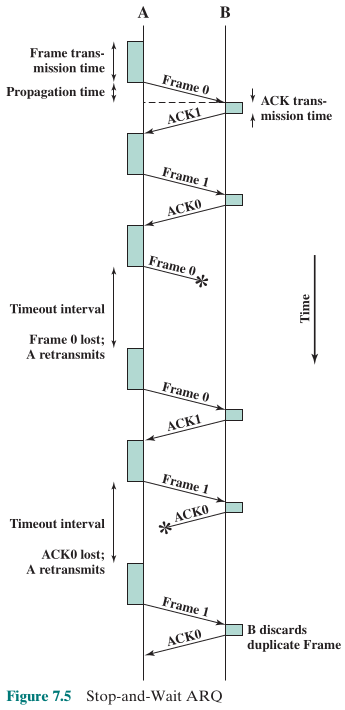
\includegraphics[height=0.9\textheight]{img/img05}
		\end{center}
		\begin{itemize}
			\item see example with both types of errors
			\item pros and cons
			\begin{itemize}
				\item simple
				\item inefficient
			\end{itemize}
		\end{itemize}
		\vfill\null
	\end{multicols}
\end{frame}

\begin{frame}
	\frametitle{Go-Back-N ARQ}
	\begin{itemize}
		\item Most commonly used error control
		\item Based on sliding-window
		\item Use window size to control number of outstanding frames
		\item While no errors occur, the destination will acknowledge incoming frames as usual
		\begin{itemize}
			\item RR=receive ready, or piggybacked acknowledgment
		\end{itemize}
		\item If the destination station detects an error in a frame, it may send a negative acknowledgment
		\begin{itemize}
			\item REJ=reject
			\item Destination will \textbf{discard that frame and all future frames until the frame in error is received correctly}
			\item Transmitter must \textbf{go back and retransmit} that frame and all subsequent frames
		\end{itemize}
	\end{itemize}
\end{frame}

\begin{frame}
	\frametitle{Summary}
	\begin{multicols}{2}
	\begin{itemize}
		\item Types of errors
		\item Error detection
		\item Parity check
		\begin{itemize}
			\item Parity bit
			\item Two-dimensional parity check
		\end{itemize}
		\item Internet checksum
		\item Cyclic redundancy check
		\begin{itemize}
			\item Modulo 2 arithmetic
			\item Polynomials
			\item Digital logic
		\end{itemize}
		\item Forward error correction
		\begin{itemize}
			\item Block code principles
		\end{itemize}
	\end{itemize}
	\end{multicols}
\end{frame}

\begin{frame}
	\frametitle{Tugas Mandiri}
	\begin{itemize}
		\item Stallings, W. (2014). Data and Computer Communications, 10th Edition, New Jersey: Upper Saddle River
		\begin{itemize}
			\item Chapter 6 Error Detection and Correction
		\end{itemize}
		\item Gupta, P. C. (2006). Data Communications and Computer Networks. New Delhi: Prentice Hall of India
		\begin{itemize}
			\item Chapter 5 Error Control
		\end{itemize}
		\item Tanenbaum, A. S. \& Wetherall, D. J. (2013). Computer Networks, Fifth Edition. London: Pearson.
		\begin{itemize}
			\item Section 3.2 Error Detection and Correction
		\end{itemize}
	\end{itemize}
\end{frame}

\begin{frame}
	\frametitle{Tugas Terstruktur}
	\textbf{Tampilkan Tugas 5}
\end{frame}

\end{document}
